\pdfinfo{
/ModDate (\pdfcreationdate)                                   
/Producer (pdfLaTeX)                                    
}


\documentclass[fleqn,oneside,openany,a4paper,11pt]{book}

\usepackage{color}
\usepackage[utf8]{inputenc}
\usepackage[breaklinks]{hyperref} %
\usepackage{pracadok}
\usepackage{longtable}
\usepackage{hyperref}
\usepackage{sidecap}
\usepackage{graphicx}
\usepackage{wrapfig}
%\usepackage{array}
%\usepackage{geometry}
%\usepackage{fancyhdr}
\usepackage{float}

\pdfcompresslevel=9

\def\uwaga#1{}

\begin{document}
\let\s\lstinline
\lstset{inputencoding=utf8, extendedchars=true,literate={ą}{{\k{a}}}1 {ć}{{\'c}}1 {ę}{{\k{e}}}1 {ł}{{\l{}}}1 {ń}{{\'n}}1 {ó}{{\'o}}1 {ś}{{\'s}}1 {ż}{{\.z}}1 {ź}{{\'z}}1 {Ą}{{\k{A}}}1 {Ć}{{\'C}}1 {Ę}{{\k{E}}}1 {Ł}{{\L{}}}1 {Ń}{{\'N}}1 {Ó}{{\'O}}1 {Ś}{{\'S}}1 {Ż}{{\.Z}}1 {Ź}{{\'Z}}1}

% Tytuł

\def\autor{Informatyka Stosowana III rok}
\def\tytul{\textbf{\LARGE Zespołowe Przedsięwzięcie Inżynierskie}}
\def\promotor{~}
\def\miejscerokwydania{Nowy Sącz \today}
\def\nazwauczelni{PAŃSTWOWA WYŻSZA SZKOŁA ZAWODOWA}
\def\imienia{INSTYTUT  TECHNICZNY}
\def\wydzial{Kierunek Informatyka Stosowana}
\begin{figure}[H]
\centering

\includegraphics[scale=0.3]{czlonkowie/fig/logo.png}
\end{figure}
\thispagestyle{empty}
{
\hbox{}\vskip 0.1\textheight
\hspace{0.1cm}
\centering
\vbox{
\noindent\textbf{\Huge Nadanie cech lokalizacji książek,  znajdujących się w czytelni PWSZ w Nowym Sączu}\\
\vspace{0.5cm}
\noindent\textbf{\vspace{0.5cm}\huge Zespołowe przedsięwzięcie inżynierskie}\\
\noindent\textbf{\huge Prowadzący: Antoni Ligęza}}\\}
%\noindent e-mail: \verb|aligeza@pwsz-ns.edu.pl|\\
%\noindent \verb|http://www.pwsz-ns.edu.pl/aligeza|}\\}



\definecolor{tlo}{rgb}{.7,.7,.7} 
\lstset{language=bash,commentstyle=\scriptsize,backgroundcolor=\color{tlo},%
basicstyle=\scriptsize}

%spis tresci
{\footnotesize\tableofcontents}

\setcounter{chapter}{0}
%Opis wykonywanego zadania
%Cel
%Zakres prac

\flushleft \chapter{Zespołowe przedsięwzięcie}

\begin{itemize}
\item Zespołowe przedsięwzięcie inżynierskie oznaczać będzie projekt, działanie podjęte w realizacji postawionego celu, realizowane zespołowo.

\item Projekt jest odpowiedzią na problem/potrzebę, w określonej przestrzeni życia.
\end{itemize}

\section{Członkowie zespołu z określeniem funkcji}
\begin{description}
\item[1] Krzysztof Szabla - kierownik zespołu
\item[2] Mateusz Kempa - programista 
\item[3] Robert Dudzik - programista
\item[4] Adam Walczak - testujący
\end{description}

\section{Uzasadnienie potrzeby realizacji projektu}

Projekt obejmuje stworzenie aplikacji GPS na Androida, która poprowadzi członków spółki leśnej do oznaczonego drzewa, przeznaczonego do wycinki. Głownym problemem dla członków spółki leśnej jest kłopot ze znalezieniem trasy dojścia do danego drzewa, które wcześniej oznaczyli. Program ma powstać w celu uwydatnienia pracy spółki leśnej, członkowie będą wprowadzać punkty, czyli współrzędne oznaczonych drzew,  na podstawie których aplikacja będzie kierować ich w odpowiednie miejsce. Ich praca zostanie wykonana znacznie szybciej. Odpowiedzią na  rozwiązanie problemu będzie zespołowo zrealizowany projekt, którego wynikiem końcowym będą: program i sporządzona dokumentacja.

\section{Cele projektu} 

 Zespołowe Przedsięwzięcie Inżynierskie obejmuje stworzenie działającej aplikacji GPS na Androida, umożliwiającej poprawne i szybkie odnalezienie wyznaczonego celu. W tym przypadku celem jest określone drzewo, przeznaczone do wycinki, które należy oznaczyć odpowiednimi współrzędnymi, tak by członkowie spółki leśnej w łatwy sposób mogli je odnaleźć. Aplikacja ma wskazać trasę dojścia do oznaczonych wcześniej  obiektów..
 
 Główne cele:
 \begin{itemize} 
 \item zapoznanie się z zestawem Android SDK i odpowiednią literaturą przez programistów 
 \item wyszukanie podobnych do projektowanej aplikacji typu opensource i zapoznanie z nimi
 \item stworzenie działającej aplikacji i przetestowanie jej pod kątem zgodności z wytyczonymi zadaniami
 \item sporządzenie dokumentacji przez każdego członka zespołu na temat pracy jaką wykonał
 \end{itemize}

\section{Zakres projektu}
Zakres projektu obejmuje podzielenie obowiązków pomiędzy członków zespołu,  wyszukanie potrzebnych informacji i przygotowanie odpowiednich narzędzi. W celu rozpoczęcia pracy przy projekcie należy zapoznać się z literaturą i skorzystać z oprogramowania typu opensource w celu zapoznania się z kodem podobnych aplikacji. Do rozpoczęcia projektu potrzebne będą dwie rzeczy:Java Developer Kit, oraz zestaw Android SDK.  Android SDK zawiera kompilator programów na platformę Android, narzędzia do tworzenia i zarządzania wirtualnymi urządzeniami (na których możemy testować nasze programy), a także środowisko programistyczne Eclipse, JDK to  Java z narzędziami dla programistów (np. kompilator Javy).Zadaniem programistów jest napisanie programu, który zostanie przetestowany przez testera, by wyeliminować ewentualne błędy.
Projekt obejmuje także sporządzenie dokumentacji na temat wykonanej pracy.

\section{Grupy docelowe}

Głównymi odbiorcami i użytkownikami projektu są członkowie spółki leśnej, zajmujący się wycinką drzew.

\section{Struktura podziału prac (zadań) - WBS}

\begin{enumerate}
\item Wybór tematu projektu.
\item Wywiad ze zleceniodawcą i zebranie informacji na temat wymagań związanych z aplikacją.
\item Podzielenie zadań pomiędzy członków zespołu i zapoznanie z tematem.

- informacje o celu projektu

- informacje na temat działania programu

- informacje o wyniku, jaki ma być zwrócony przez program
\item Przygotowanie odpowiednich narzędzi i gromadzenie niezbędnych danych.

- przygotowanie środowiska Latex

- przygotowanie środowiska Android Studio
\item Napisanie programu.

-zaplanowanie interakcji pomiędzy poszczególnymi elementami aplikacji

-tworzenie algorytmów

-opis interfejsu

\item Testowanie programu i wprowadzanie ewentualnych zmian.
\end{enumerate}

\section{Diagram sieciowy}
Diagram sieciowy ukazuje zależności czasowe, węzły (aktywności), krawędzie (zależności czasowe).
\begin{figure}[H]
\centering
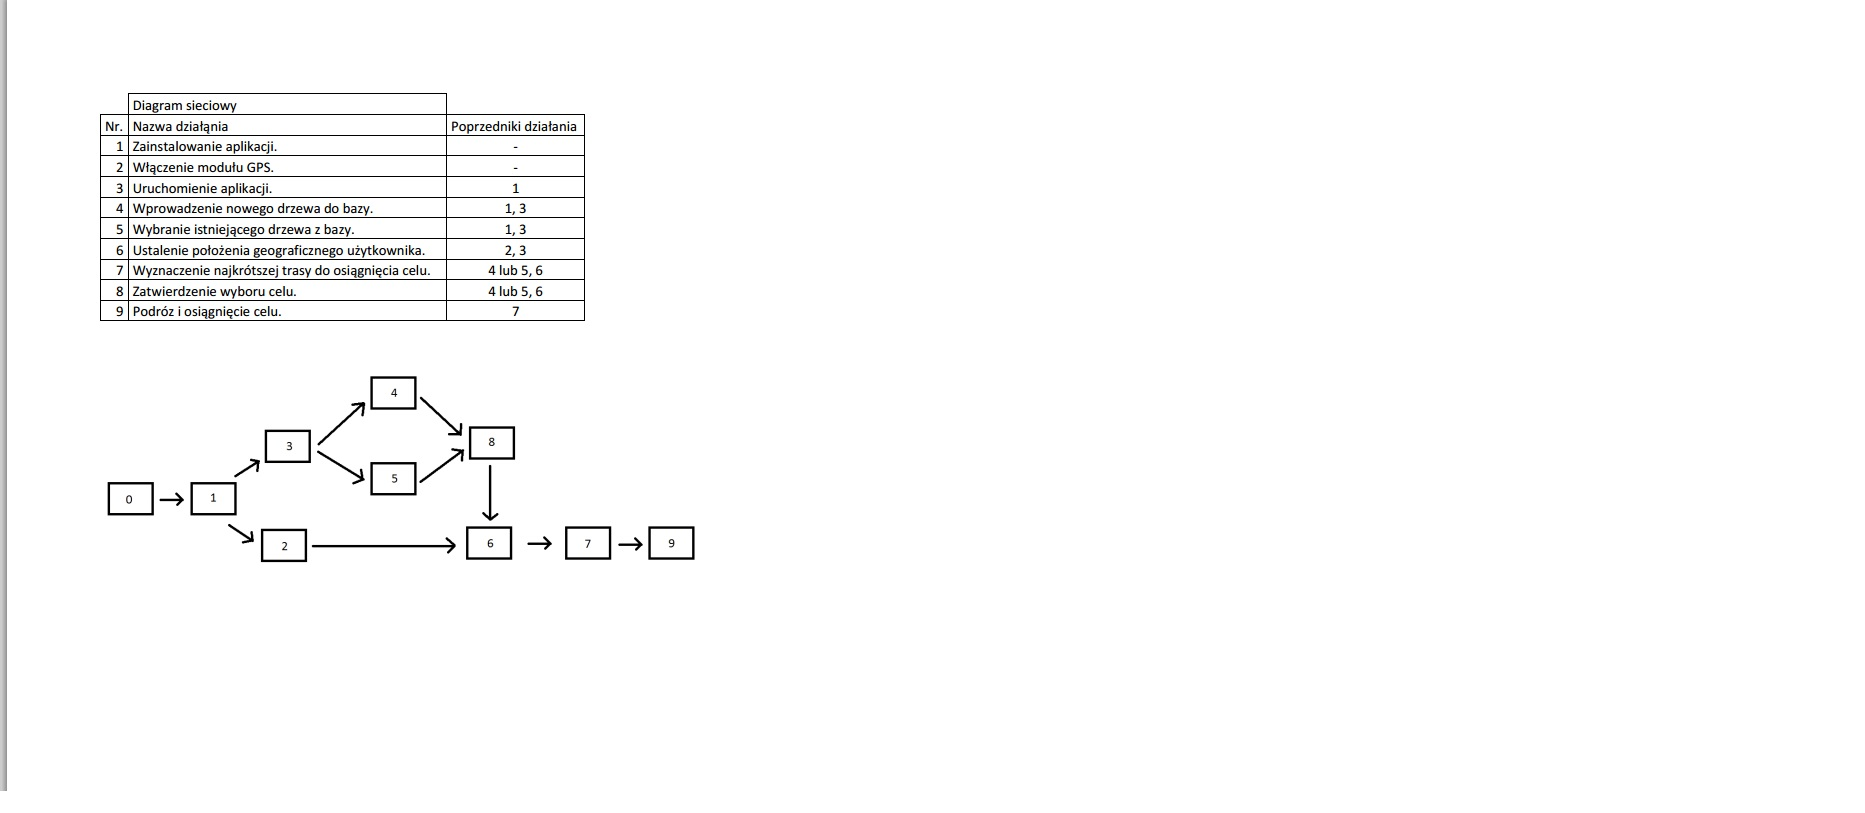
\includegraphics[scale=0.5]{czlonkowie/fig/diagram.jpg}
\end{figure}

\section{Harmonogram}
\begin{figure}[H]
\centering
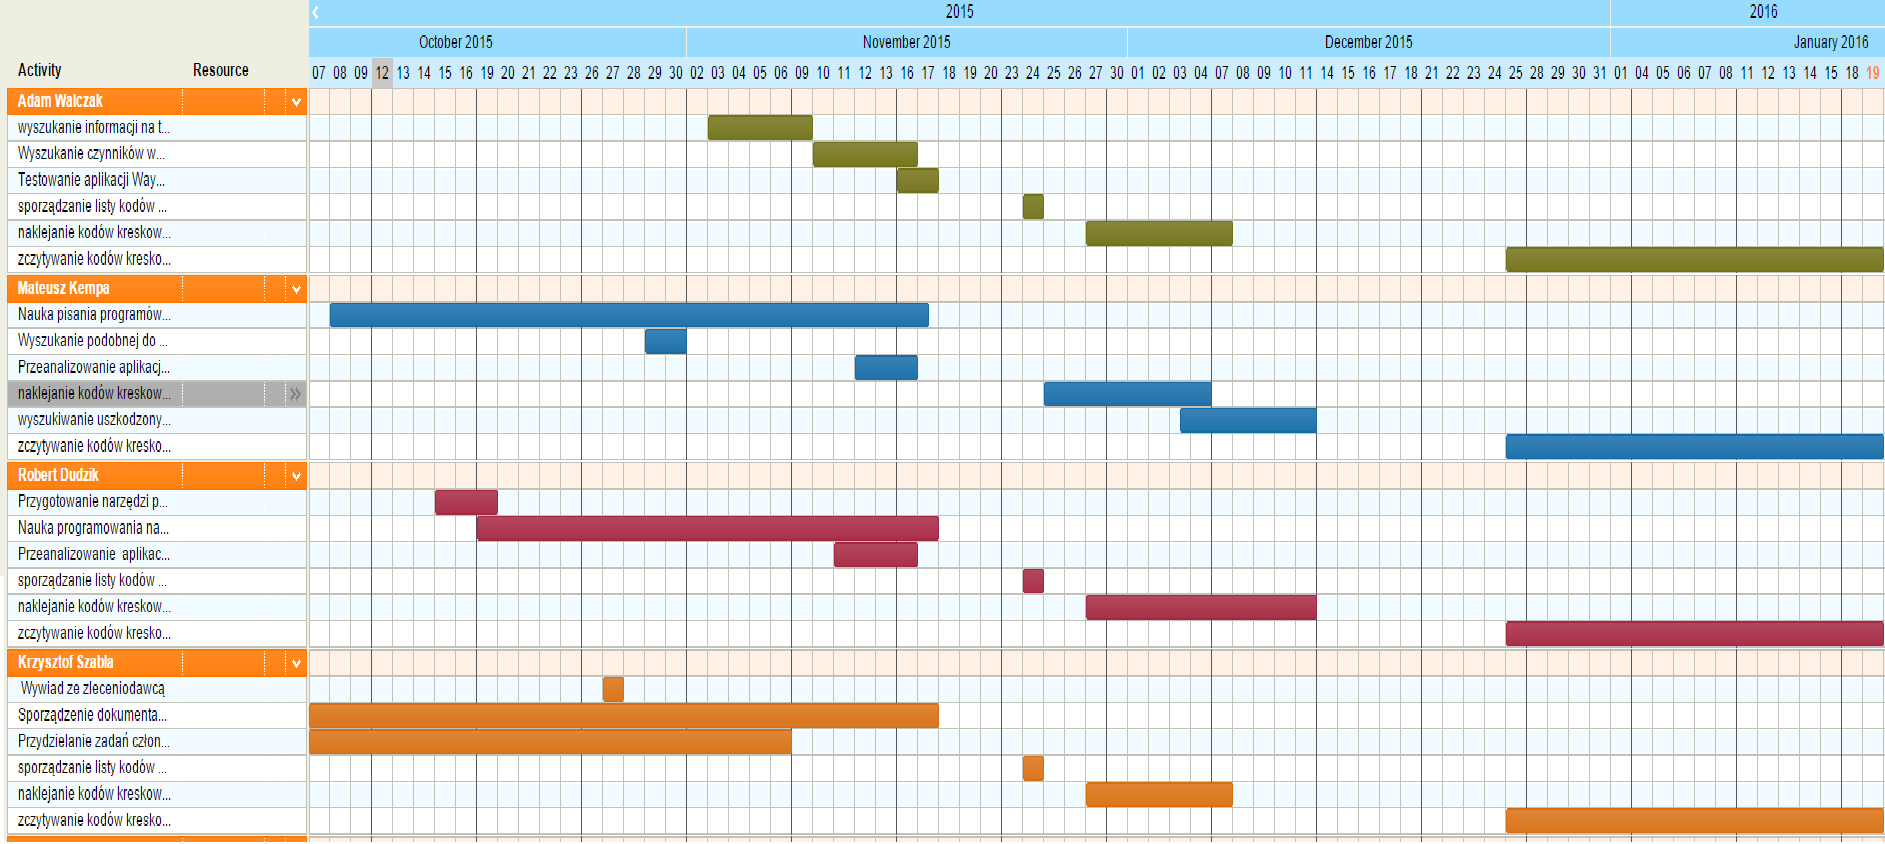
\includegraphics[scale=0.5219 , angle=90,]{czlonkowie/1/wykresGantta.png}

\end{figure}




\subsection{Harmonogram prac poszczególnych członków zespołu}

 Adam Walczak- tester. \newline
 
\textbf{GPS}
\begin{itemize}
\item Wyszukanie informacji na temat dokładności GPS-a.

\textbf{Data rozpoczęcia} 03.11.2015

\textbf{Data zakończenia} 10.11.2015
\item Wyszukanie czynników wpływających na wynik pomiaru GPS, wad i zalet GPS

\textbf{Data rozpoczęcia} 10.11.2015

\textbf{Data zakończenia} 16.11.2015
\item Testowanie aplikacji Waypoint w terenie.

\textbf{Data rozpoczęcia} 16.11.2015

\textbf{Data zakończenia} 17.11.2015
 \newline

\textbf{Biblioteka}
\item sporządzanie listy kodów kreskowych

\textbf{Data rozpoczęcia} 24.11.2015

\textbf{Data zakończenia} 24.11.2015

\item naklejanie kodów kreskowych na regałach  w czytelni

\textbf{Data rozpoczęcia} 27.11.2015

\textbf{Data zakończenia} 07.12.2015

\item zczytywanie kodów kreskowych książek w czytelni

\textbf{Data rozpoczęcia} 25.12.2015 

(w trakcie realizacji)

\end{itemize}

Mateusz Kempa- programista

\textbf{GPS}
\begin{itemize}
\item Nauka pisania programów na Androida


\textbf{Data rozpoczęcia} 08.10.2015

\textbf{Data zakończenia} 17.11.2015
\item  Wyszukanie podobnej do zadanej aplikacji, którą można wykorzystać przy projekcie.

\textbf{Data rozpoczęcia} 29.10.2015

\textbf{Data zakończenia} 31.10.2015

\item Przeanalizowanie aplikacji Waypoint i określenie w jakim stopniu będzie pomocna przy projekcie

\textbf{Data rozpoczęcia} 12.11.2015

\textbf{Data zakończenia} 16.11.2015

\item naklejanie kodów kreskowych na regałach  w czytelni

\textbf{Data rozpoczęcia} 28.11.2015

\textbf{Data zakończenia} 05.12.2015

\item wyszukiwanie uszkodzonych kodów kreskowych

\textbf{Data rozpoczęcia} 03.12.2015

\textbf{Data zakończenia} 12.12.2015

\item zczytywanie kodów kreskowych książek w czytelni

\textbf{Data rozpoczęcia} 25.12.2015 

(w trakcie realizacji)
 \end{itemize}
 
 
 Robert Dudzik- programista
 
 \textbf{GPS}
 
 \begin{itemize}
 \item Przygotowanie narzędzi programistycznych Android Studio
 
 \textbf{Data rozpoczęcia} 15.10.2015

\textbf{Data zakończenia} 19.10.2015

\item Nauka programowania na Androidzie na podstawie dostępnej literatury i stron internetowych

\textbf{Data rozpoczęcia} 19.10.2015

\textbf{Data zakończenia} 17.11.2015

\item Przeanalizowanie  aplikacji Waypoint i określenie w jakim stopniu będzie pomocna przy projekcie

\textbf{Data rozpoczęcia} 11.11.2015

\textbf{Data zakończenia} 16.11.2015


\textbf{Biblioteka}

\item sporządzanie listy kodów kreskowych

\textbf{Data rozpoczęcia} 24.11.2015

\textbf{Data zakończenia} 24.11.2015
\item naklejanie kodów kreskowych na regałach  w czytelni

\textbf{Data rozpoczęcia} 27.11.2015

\textbf{Data zakończenia} 11.12.2015

\item zczytywanie kodów kreskowych książek w czytelni

\textbf{Data rozpoczęcia} 25.12.2015

(w trakcie realizacji)
 \end{itemize}

Krzysztof Szabla- kierownik zespołu

\textbf{GPS}
\begin{itemize}

\item Wywiad ze zleceniodawcą

\textbf{Data rozpoczęcia} 27.10.2015

\textbf{Data zakończenia} 27.10.2015
\item Sporządzenie dokumentacji

\textbf{Data rozpoczęcia} 07.10.2015

\textbf{Data zakończenia} 17.11.2015

\item  Przydzielanie zadań członkom zespołu

\textbf{Data rozpoczęcia} 07.10.2015

\textbf{Data zakończenia} 06.11.2015

\textbf{Biblioteka}

\item sporządzanie listy kodów kreskowych

\textbf{Data rozpoczęcia} 24.11.2015

\textbf{Data zakończenia} 24.11.2015 



\item naklejanie kodów kreskowych na regałach  w czytelni

\textbf{Data rozpoczęcia} 28.11.2015

\textbf{Data zakończenia} 07.12.2015


\item zczytywanie kodów kreskowych książek w czytelni

\textbf{Data rozpoczęcia} 25.12.2015 

(w trakcie realizacji)


\end{itemize}

\section{Zmiana tematu}

Dnia 17 listopada nastąpiła zmiana tematu projektu. Przyczyną była duża trudność poprzedniego projektu i problemy programistyczne. Nowy temat to: ,,Nadanie cech lokalizacji książek,  znajdujących się w czytelni PWSZ w Nowym Sączu''. Dzięki jego realizacji, czytelnik po odnalezieniu książki w katalogu elektronicznym, będzie w stanie z dokładnością do półki, odnaleźć fizyczny egzemplarz książki. 

\section{Cele nowego projektu} 
~~~Zespołowe przedsięwzięcie inżynierskie obejmuje stworzenie systemu, który umożliwi czytelnikowi odnalezienie fizycznej lokalizacji książki wyszukanej w elektronicznym katalogu biblioteki PWSZ. 

~~~Na wstępie należy sprawdzić, jakimi czytnikami dysponuje czytelnia i wybrać kod kreskowy. W naszym projekcie używany będzie Code 39, ponieważ jest on obsługiwany przez czytniki znajdujące się w bibliotece oraz koduje znaki alfanumeryczne wraz ze znakami specjalnymi (takimi jak znak pauzy). Każdy kod będzie składał się z dwóch liczb całkowitych. Pierwsza to numer regału, a druga numer półki. Oddzielał je będzie znak '-'. Numeracja zaczyna się od '1-1' w górę, by w razie potrzeby można było rozbudować regał o kolejne półki. 

~~~Następnie trzeba będzie przygotować szablon kodów kreskowych, tak by były one odpowiedniej wielkości i jak najwięcej zmieściło się ich na jednej stronie. Na podstawie rozmiarów półek ustaliliśmy, że kody powinny mieć wysokość 13 mm, a margines z prawej strony wynosić 6 mm. Do utworzenia szablonu użyjemy programu Microsoft Excel oraz darmowej czcionki o nazwie "fre3of9x". 

~~~W dalszej kolejności zajmiemy się wydrukiem kodów. W tym celu użyjemy przygotowanego wcześniej szablonu, który będzie drukowany na specjalnym papierze samoprzylepnym w formacie A4. Dzięki temu w prosty sposób umieścimy kody na regałach. Po wydrukowaniu, kody zostaną pocięte przy pomocy biurowej gilotyny. 

\begin{figure}[H]
\begin{center}

\includegraphics[scale=0.7]{czlonkowie/1/b2.jpg}
\caption{Przykładowy kod kreskowy}
\end{center}
\end{figure}
~~~Dalej konieczne będzie naklejenie kodów kreskowych. Umieszczać będziemy je z lewej strony półki, by później łatwo można było odczytać kody z poszczególnych książek. Każdy kod po przylepieniu musi zostać zabezpieczony przed fizycznym uszkodzeniem. Do tego wykorzystamy samoprzylepną folię ochronną, używaną w bibliotece do zabezpieczania książek lub dokumentów. Arkusz takiej folii zostanie podzielony na części o wymiarach 5x7 cm oraz 5x8.5 cm, w taki sposób aby przylepiona folia pokrywała w całości poprzednio naklejony kod. Niezwykle ważne będzie też sprawdzenie kodu już po jego zabezpieczeniu czy przypadkiem nie został on zamazany lub w jakikolwiek inny sposób uszkodzony. 

\begin{figure}[H]
\begin{center}
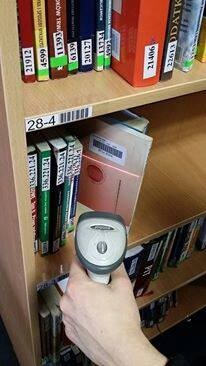
\includegraphics[scale=0.7]{czlonkowie/1/b1.jpg}
\caption{Zczytywanie kodów z książek}
\end{center}
\end{figure}

~~~Ostatnim celem naszego przedsięwzięcia jest odczytanie kodów kreskowych z książek w czytelni i przypisanie tych kodów do odpowiednich półek, w jak najbardziej efektywny sposób. Jest to jeden z najważniejszych etapów projektu. Do realizacji tego zadania posłuży nam czytnik Motorola LS2208 z interfejsem USB dostępny w bibliotece. Pozwala on odczytać kod i automatycznie zapisać go do pliku tekstowego. Kody kreskowe, które będziemy czytać znajdują się zwykle w lewym górnym rogu na tylnej stronie okładki książki. Kody te zostaną zapisane w formie listy, w notatniku. Jeśli którejś z książek nie będzie w danym momencie na półce, bo korzystali z niej czytelnicy, zostanie ona później uzupełniona przez pracowników biblioteki.
Należy tutaj sprecyzować znaczenie "najbardziej efektywnego sposobu". Nasza grupa ma za zadanie opracować system odczytu kodów, który pozwoli zrealizować ten cel w najkrótszym możliwym czasie, jednocześnie zachowując poprawność skanowanych kodów w pliku tekstowym. Opiszmy więc sposób zczytywania, który będzie sposobem optymalnym. Nasz zespół liczy czterech członków. Zakładając, że dysponujemy dwoma laptopami oraz skanerami podzielimy go na dwuosobowe podzespoły. W każdym podzespole jedna osoba zajmować się będzie zczytywaniem kodów, a druga kontrolą błędów w pliku tekstowym. Zczytywanie będzie się odbywać w następujący sposób. Najpierw pierwsza osoba skanowanć będzie kod półki, a później, od lewej strony wszystkie książki znajdujące się na poszczególnej półce. Przykładowy fragment pliku .txt będzie więc wyglądać tak: 
\begin{lstlisting}
88-1
88-2
0490000060045
0490000054227
0490000060046
0490000060036
0490000073645
0490000060047
0490000058234
0490000047888
0490000054041
88-3
0490000071851
0490000059162
\end{lstlisting}
Jak widzimy w pierwszym wierszu znajduje się kod półki '88-1'. Na tej półce nie znajdują się żadne książki, więc w kolejnym wierszu pojawia się kod następnej półki. Pod nim lista książek z owej półki. Dalej plik jest uzupełniany w podobny sposób. W tym samym czasie  druga osoba musi nieustannie monitorować zczytywane kody w pliku tekstowym, aby w razie nieudanego/niepoprawnego odczytu można było go powtórzyć. Druga podgrupa, wykorzystując identyczną metodę, zczytuje kody z innego regału. Warto w tym miejscu wspomnieć o pomiarach, które wykonaliśmy. Uśredniony czas zczytywania kodów z jednej półki wyniósł: 55.5 sekundy, natomiast jednego regału:5 minut 30 sekund.
Testowaliśmy również inny system skanowania, który w skrócie wyglądał tak: trzyosobowa grupa pracowała razem, pierwsza osoba zdejmowała i układała książki na półkach, druga zczytywała kody, a trzecia kontrolowała poprawność w pliku tekstowym. Średni czas skanowania półki dla tego sposobu to: 64.55 sekund, a regału: 6 minut 24 sekundy
Łatwo zauważyć, iż pierwszy system zczytywania jest lepszy od drugiego, bo:
\begin{itemize}
\item Jest on przeznaczony dla czteroosbowej grupy, tak więc wykorzystamy jej potencjał w pełni
\item Średni czas skanowania jest mniejszy - metoda jest szybsza
\item Dwie podgrupy pracują równolegle co znacznie skróci czas wykonywania zadania.
\end{itemize}
Jedyną zaletą drugiego systemu jest szybsze skanowanie książek na przepełnionych półkach, problematycznych w skanowaniu dla jednej osoby.

\section{Zakres nowego projektu}
Zakres nowego projektu obejmuje:

\begin{enumerate}
\item Wybór kodu kreskowego, który zostanie wykorzystany do identyfikacji regałów w czytelni. 
\item Przygotowanie szablonu kodów kreskowych w ustalonym standardzie, gotowego do druku.
\item Przylepienie kodów kreskowych na półki w czytelni PWSZ. 
\item Odczytanie kodów kreskowych wszystkich książek znajdującyh się w czytelni i przypisanie ich do odpowiednich półek (regałów).
 \end{enumerate}

\section{Grupy docelowe nowego projektu}

W nowym projekcie głównymi odbiorcami i użytkownikami są pracownicy  biblioteki oraz czytelnicy.

\section{Struktura podziału prac (zadań) - WBS dla nowego projektu}
\begin{enumerate}
\item Otrzymanie nowego tematu projektu.
\item Wywiad ze zleceniodawcą i zebranie informacji na temat wymagań związanych z projektem
\item Podzielenie zadań pomiędzy członków zespołu i zapoznanie z tematem.
\item Przygotowanie listy kodów kreskowych oraz numeracji poszczególnych półek i regałów
\item Naklejanie kodów kreskowych na regały w czytelni i zabezpieczanie ich za pomocą folii ochronnej
\item Odczytywanie kodów kreskowych książek i przypisywanie ich do odpowiedniej półki
\end{enumerate}

\section{Dokumentacja}
Przygotowanie środowiska do równoległego opracowania dokumentacji projektu i realizacji przydzielonych zadań poszczególnym członkom zespołu projektowego.

\subsection[Edycja plików dokumentacyjnych]{Edycja plików dokumentacyjnych - każdy członek zespoły niezależnie}
Każdy z członków zespołu edytuje swój plik \LaTeX{} (czlonkowie/nrCzlonka/main.tex) i~umieszcza w nim całość analiz i wyników, które pozwoliły mu zrealizować przydzielone zadanie. Wszystkie pliki graficzne, każdy niezależnie umieszcza w swoim katalogu (czlonkowie/nrCzlonka).

Pierwszą linia w pliku (czlonkowie/nrCzlonka/main.tex), zawiera imię i nazwisko opracowującego członka zespołu:
\begin{lstlisting}
\osoba{Robert Dudzik}
\end{lstlisting}

Każde działanie/zadanie należy DOKŁADNIE opisać podając w poleceniu \s!\zadanieprojektowe! cztery obowiązkowe dane:
\begin{itemize}
\item Rodzaj zadania [Przygotowanie przestrzeni do zespołowej pracy]
\item Data rozpoczęcia [2015-10-06]
\item Data zakończenia [2014-11-02]
\item Aktualny status [zaplanowane do realizacji]
\item dokładny opis realizowanego zadania [powinien zawierać opis, rysunki, tabele, kody napisanych programów]
\end{itemize}

Poniżej znajduje się przykładowy listing dla skróconych dwóch zadań:
\begin{lstlisting}
\zadanieprojektowe{Przygotowanie dokumentacji}{2014-11-01}{2014-11-02}{w trakcie do realizacji}

Poniżej opisujemy całe zadanie zgodnie z konwencją poznaną na NI.
Poniżej opisujemy całe zadanie zgodnie z konwencją poznaną na NI.

Poniżej opisujemy całe zadanie zgodnie z konwencją poznaną na NI. 

%następne zadanie
\zadanieprojektowe{Przygotowanie dokumentacji}{2014-11-03}{2014-11-03}{zakończone}
\begin{figure}[H]
\includegraphics[width=\textwidth]{czlonkowie/1/studzienkizDziura.jpg}
\end{figure}
\end{lstlisting}


\subsubsection{Obsługa SVN}
Umieszczanie w repozytorium plików lub katalogów dotychczas nie podlegający zarządzaniu wersjami.

Użycie: import [ŚCIEŻKA] URL

Rekurencyjnie kopiuje ŚCIEŻKA do URL. Jeśli ŚCIEŻKA nie jest podana, domyślną wartością jest '.'. W repozytorium są w razie potrzeby tworzone brakujące katalogi nadrzędne. Jeśli argument ŚCIEŻKA jest katalogiem, to zawartość katalogu jest dodawana bezpośrednio za URL-em.

Przydatne parametry:

-m ARG  -  użyj podanego tekstu jako opisu zmian

--username ARG  : użyj ARG jako nazwy użytkownika

--password ARG  : użyj ARG jako hasła

Tworzenie kopii roboczej projektu

Użycie: checkout URL[@WERSJA]... [ŚCIEŻKA]

Pobiera dane z URL i umieszcza je w ŚCIEŻKA.

Dodawanie i aktualizacja plików/katalogów

Użycie: commit [ŚCIEŻKA...]

Zatwierdza zmiany dokonane na kopii roboczej zapisując je w repozytorium. ŚCIEŻKA wskazuje pliki/katalogi z kopii roboczej, które mają być uaktualnione w repozytorium.

Aktualizacja kopi roboczej projektu

Użycie: update [ŚCIEŻKA...]

Aktualizuje kopię roboczą nanosząc zmiany obecne w repozytorium.  Jeśli nie podano wersji, nanoszone są najnowsze zmiany z  repozytorium (wersja HEAD).

%Jan Kowalski - kierownik zespołu

\osoba{Krzysztof Szabla}
\zadanieprojektowe{Wyszukanie potrzebnych narzędzi i literatury.}{2015-10-14}{2015-10-20}{zakończone}



Do rozpoczęcia projektu potrzebne będą dwie rzeczy:Java Developer Kit, oraz zestaw Android SDK.  Android SDK zawiera kompilator programów na platformę Android, narzędzia do tworzenia i zarządzania wirtualnymi urządzeniami (na których możemy testować nasze programy), a także środowisko programistyczne Eclipse, JDK to po  Java z narzędziami dla programistów (np. kompilator Javy). W pierwszej kolejności pobieramy i instalujemy JDK. Możemy je pobrać ze strony http://www.oracle.com/technetwork/java/javase/downloads/index.html. Po pobraniu i rozpakowaniu, w rozpakowanym katalogu są katalogi eclipse, sdk, oraz program SDK Manager. 
By zapoznać się z literaturą potrzebną do napisania aplikacji wyszukałem kilka pozycji w bibliotece takich jak:  "Android : aplikacje wielowątkowe, techniki przetwarzania"  Anders Göransson czy "Android : tworzenie aplikacji w oparciu o HTML, CSS i JavaScript"  Jonathan Stark, Brian Jepson i "Android-programowanie aplikacji na urządzenia przenośne" Shane Conder.
\zadanieprojektowe{Wywiad ze zleceniodawcą}{2015-10-14}{2015-10-20}{zakończone}
Celem przeprowadzenia wywiadu było zdobycie informacji na temat celu stworzenia aplikacji i grup odbiorców, dla której przeznaczona jest aplikacja, czyli spółki leśnej
\zadanieprojektowe{Czytniki kodów kreskowych. Sporządzenie listy kodów kreskowych do czytelni}{2015-11-20}{2015-11-21}{zakończone}
W polskich bibliotekach rośnie zapotrzebowanie na kody kreskowe. W bibliotekach (szkolnych, uniwersyteckich i publicznych) coraz częściej są wydawane karty czytelnika z kodem kreskowym, kody kreskowe są również naklejane na woluminy. Autoryzowanie czytelników przez kody kreskowe w pewnym stopniu uniemożliwia podszywanie się pod innych czytelników (oprogramowanie komputerowe coraz częściej oferuje zapisywanie w systemie zdjęć czytelników). Naklejanie kodów na woluminy i rejestrowanie ich w specjalnym oprogramowaniu ułatwia rejestrację wypożyczeń w systemie.

Rodzaje skanerów:

Początkowo skanery kodów używały diod LED jako źródła światła. Wadą tego rozwiązania była konieczność zbliżenia skanera na bardzo małą odległość od kodu. Obecnie produkowane skanery używają lasera, co umożliwia - zależnie od modelu - odczyt nawet z kilku metrów. Nowoczesne skanery potrafią odczytywać nie tylko kody jednowymiarowe (paskowe), lecz także kody 2D - dwuwymiarowe np. QR Code, Aztec Code oraz PDF417. Również prawie każdy nowy telefon posiadający kamerę można wyposażyć w odpowiednią aplikację, służącą do odczytu kodów kreskowych.

Naszym zadaniem było sporządzenie listy kodów kreskowych, którymi zostaną oznaczone półki w regałach z książkami w czytelni. Oznaczenie musi być odpowiednio dobrze widoczne  przez czytelników i pracowników biblioteki. 
Sporządziliśmy listę kodów kreskowych dla 90 regałow po 7 półek w każdym.

Do testowania działania kodów kreskowych używaliśmy skanera Motorola LS2208.


Używany kod kreskowy to Code 39, jest to  alfanumeryczny kod kreskowy o stałej szerokości pojedynczego znaku. Kod ten powstał w 1974 roku, a rozpowszechnił się po zastosowaniu go przez Departament Obrony USA do oznaczania przesyłek od dostawców. Obecnie jest wykorzystywany w branży motoryzacyjnej do oznaczania części. Największą wadą kodu jest stosunkowo mała gęstość zapisu danych. Z tego względu kod ten nie nadaje się do umieszczania na małych przedmiotach. Zaletą kodu jest fakt, iż może on zostać odczytany przez prawie każdy czytnik kodów kreskowych.

\zadanieprojektowe{Naklejanie kodów kreskowych na regałach w czytelni}{2015-11-07}{2015-12-05}{}{zrealizowano}

Naszym kolejnym zadaniem było naklejenie wszystkich kodów kreskowych typu Code 39 wraz z oznaczeniami numerycznymi na 6 półek w każdym regale, a następnie pokrycie tych kodów  specjalnymi foliami ochronnymi o wymiarach 5x7cm i 5x8,5cm. Do oznaczenia było 100 regałów.

\zadanieprojektowe{Odczytywanie kodów kreskowych książek i przypisywanie ich do półek w czytelni}{2015-12-11}{}{w trakcie realizacji}

Naszym następnym zadaniem było odczytanie przy pomocy czytnika Motorola LS2208 kodów kreskowych z książek znajdujących się w czytelni, a następnie przypisanie ich do odpowiednich półek i zapisanie listy kodów w notatniku.%Jan Nowicki
\osoba{Mateusz Kempa}

\zadanieprojektowe{Przegląd aplikacji open source}{2015-10-29}{2015-10-31}{zakończone}

Poszukiwania aplikacji open source wykorzystujących GPS rozpocząłem na dwóch najpopularniejszych serwisach z otwartymi oraz darmowymi apkami na platformę Android tj., {\color{blue}\underline{\href{https://f-droid.org/repository/browse/?fdcategory=Navigation}{F-Droid}}} oraz {\color{blue}\underline{\href{https://fossdroid.com/c/navigation/whats_new.html}{Fossdroid}}}. Na tych witrynach znajduje się multum narzędzi open source służących do nawigacji w systemie Android. Niestety, wymagań projektowych nie spełnia żadne z nich. Wtedy z pomocą przyszedł Google Play. Aplikacja, którą tam znalazłem nazywa się \textbf{WayPoint} i wydaję się być przydatna z mojego punktu widzenia. Po otwarciu, WayPoint szuka sygnału GPS i jeżeli nasze urządzenie złapie fixa, można zapisać aktualne współrzędne lokalizacji, w której się znajdujemy - Add WayPoint. Kiedy już zapisaliśmy punkt(y), wybieramy żądany z menu My WayPoints. W tym momencie przechodzimy już do nawigacji. Aplikacja oblicza odległość dzielącą nas od celu oraz wyświetla jego współrzędne. Do wyboru mamy widok mapy lub wskaźnika. To wszystko. Choć opisana aplikacja jest dość prosta to można moim zdaniem wykorzystać ją do projektu. Na pewno nie obędzie się bez modyfikacji. Poniżej zamieszczam parę screenshotów oraz link do repozytorium.

\begin{figure}[H]
\centering
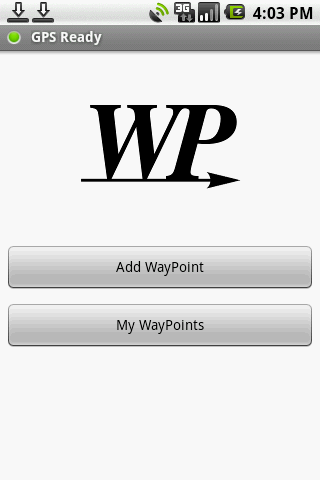
\includegraphics[scale=0.5]{czlonkowie/3/1waypoint.png}
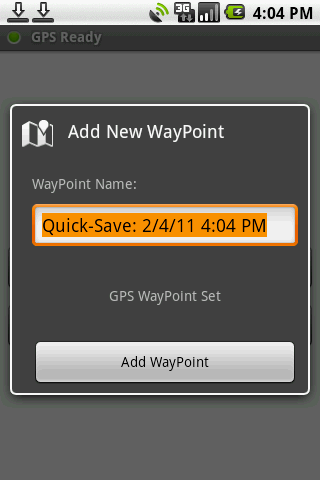
\includegraphics[scale=0.5]{czlonkowie/3/2waypoint.png}
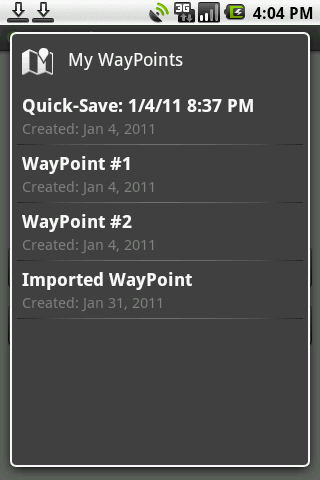
\includegraphics[scale=0.5]{czlonkowie/3/3waypoint.png}

\includegraphics[scale=0.5]{czlonkowie/3/4waypoint.png}
\end{figure}

Repozytorium: {\color{blue}\underline{\href{https://github.com/pettyjamesm/WayPoint}{github.com/pettyjamesm/WayPoint}}}
\newline \newline
Inne aplikacje open source warte uwagi: {\color{blue}\underline{\href{https://github.com/andreynovikov/Androzic}{Androzic}}}, {\color{blue}\underline{\href{https://github.com/borneq/HereGPSLocation}{HereGPSLocation}}}

\zadanieprojektowe{Przeanalizowanie aplikacji Waypoint i określenie w jakim stopniu będzie pomocna przy projekcie}{12.11.2015} {16.11.2015}{zakończone} 

\zadanieprojektowe{Wyszukiwanie uszkodzonych kodów kreskowych}{03.12.2015}{05.12.2015}{zakończone}

Podczas pierwszej wizyty w czytelni, naszym zadaniem było naklejanie części kodów kreskowych na regałach. Niestety, po naklejeniu okazało się, że niektóre kody zostały przez nieuwagę zatarte. Mogło to w przyszłości spowodować problemy z odczytem. Do moich obowiązków należało odnalezienie uszkodzonych kodów kreskowych, spisanie ich, przygotwanie gotowego do druku pliku pdf zgodnego z wymaganiami projektowymi. W czasie pierwszego spotkania projektowego w czytelni, kody kreskowe zostały naklejone na 40 regałach.

\zadanieprojektowe{Naklejanie kodów kreskowych na regałach  w czytelni}{28.11.2015}{05.12.2015}{zakończone}

Tym razem podzieliliśmy zakres obowiązków między wycinanie i naklejanie kodów oraz naklejanie folii ochronnej. Do mnie należało naklejanie kodów kreskowych oraz folii. Zdołaliśmy nakleić kody na regały 40-90. Przy wycinaniu wystąpił pewien problem i niektóre kody kreskowe uległy nie mogły zostać naklejone. Konieczne było ich spisanie, aby można było je następnym razem uzupełnić.

\zadanieprojektowe{Naklejanie kodów kreskowych na regałach w czytelni c.d.}{08.12.2015}{12.12.2015}{zakończone}

Na tym spotkaniu naszym celem było naklejenie pozostałych kodów łącznie ze wcześniej uszkodzonymi oraz zabezpieczenie ich folią. Podział obowiązków był jednak większy, gdyż tylko 2 osoby mogły się tym razem stawić w czytelni. Ja zająłem się przygotowaniem folii oraz naklejeniem części kodów. Po ukończeniu naszych zadań wszystkie kody na 102 regałach były gotowe do użycia.  

\zadanieprojektowe{Edycja dokumentacji}{08.12.2015}{}{w realizacji} 

Na podstawie przykładowej dokumentacji, zmodyfikowałem sekcje: "Cele nowego projektu" oraz "Zakres nowego projektu".

\zadanieprojektowe{Odczyt kodów kreskowych z książek}{15.12.2015}{}{w realizacji} 

Odczytaliśmy kody z książek z pierwszych 20 regałów. Moim zadaniem była kontrola odczytu i zapisu kodów kreskowych w notatniku.










%Ferdynand Sobieraj
\osoba{Robert Dudzik}
\zadanieprojektowe{Nauka programowania w Androidzie.}{2015-10-08}{2015-11-17}{zakończone}

Fragmenty kodu GPS.
\begin{lstlisting}
import android.location.Criteria;
import android.location.Location;
import android.location.LocationListener;
import android.location.LocationManager;
import android.os.Bundle;
import android.app.Activity;
import android.util.Log;
import android.view.Menu;
import android.widget.TextView;

public class MainActivity extends Activity implements LocationListener {

	TextView t1;
	TextView t2;
	TextView t3;
	TextView t4;
	
	LocationManager lm;
	Criteria kr;
	Location loc;
	String najlepszyDostawca;
	
	private void odswiez(){
		najlepszyDostawca=lm.getBestProvider(kr, true);	
		loc=lm.getLastKnownLocation(najlepszyDostawca);		
	}
	
	@Override
	protected void onCreate(Bundle savedInstanceState) {
		super.onCreate(savedInstanceState);
		setContentView(R.layout.activity_main);
		t1=(TextView) findViewById(R.id.textView1);
		t2=(TextView) findViewById(R.id.textView2);
		t3=(TextView) findViewById(R.id.textView3);
		t4=(TextView) findViewById(R.id.textView4);
		
		kr=new Criteria();
		lm=(LocationManager) getSystemService(LOCATION_SERVICE);
		odswiez();				
		lm.requestLocationUpdates(najlepszyDostawca, 1000, 1, this);
		t1.setText("najlepszy dostawca: "+najlepszyDostawca);
		t2.setText("długość geograficzna: "+loc.getLongitude());
		t3.setText("szerokość geograficzna: "+loc.getLatitude());
		t4.setText("-------historia------\n");
	}

	@Override
	public void onLocationChanged(Location location) {
		odswiez();
		t1.setText("najlepszy dostawca: "+najlepszyDostawca);
		t2.setText("długość geograficzna: "+loc.getLongitude());
		t3.setText("szerokość geograficzna: "+loc.getLatitude());
		t4.setText(t4.getText()+""+loc.getLongitude()+"/"+loc.getLatitude()+"\n");
		
	}

	@Override
	public void onProviderDisabled(String provider) {
		// TODO Auto-generated method stub		
	}

	@Override
	public void onProviderEnabled(String provider) {
		// TODO Auto-generated method stub
		
	}

	@Override
	public void onStatusChanged(String provider, int status, Bundle extras) {
		// TODO Auto-generated method stub
		
	}
}
\end{lstlisting}

\begin{lstlisting}
<?xml version="1.0" encoding="utf-8"?>
<manifest xmlns:android="http://schemas.android.com/apk/res/android" 
android:versionName="@string/version_number" package=
"com.crobot.waypoint" android:versionCode="2">
    <application android:label="@string/app_name" android:icon="@drawable/
    wp_header">
    	<uses-library android:name="com.google.android.maps" />
        <activity android:name=".HomeActivity" android:screenOrientation=
        "portrait"  android:label="@string/app_name">
            <intent-filter>
                <action android:name="android.intent.action.MAIN" />
                <category android:name="android.intent.category.LAUNCHER" />
            </intent-filter>
            <intent-filter android:label="@string/resolve_open">
            	<action android:name="android.intent.action.VIEW" />
            	<action android:name="android.intent.action.EDIT" />
            	<category android:name="android.intent.category.DEFAULT" />         
                <data android:scheme="content" android:mimeType="vnd.
                android.cursor.item/vnd.crobot.waypoint" />
                <data android:scheme="content" android:mimeType=
                "application/vnd.crobot.waypoint" />
                <data android:scheme="file" android:mimeType=
                "vnd.android.cursor.item/vnd.crobot.waypoint" />
                <data android:scheme="file" android:mimeType=
                "application/vnd.crobot.waypoint" />
				<data android:pathPattern=".*\\.waypoint" /
				>
            </intent-filter>
        </activity>
        <activity android:screenOrientation="portrait" 
        android:name=".TrackingActivity">
        	
        </activity>
        <service android:enabled="true" android:name="
        com.crobot.waypoint.tracking.WayPointSvc"/>
	</application>
    <uses-sdk android:minSdkVersion="4" android:targetSdkVersion="4"/>
    <uses-permission android:name="android.permission.INTERNET" />
	<uses-permission android:name="android.permission.ACCESS_FINE_LOCATION"/>
	<uses-permission android:name=
	"android.permission.WRITE_EXTERNAL_STORAGE" />
</manifest> 
\end{lstlisting}

\zadanieprojektowe{Przygotowanie kodów kreskowych w Excelu}{2015-11-18}{2015-11-26}{zakończone}

Przygotowaliśmy kody kreskowe w Code39 dla 102 regałów, każdy z nich składał się z 6-ciu półek. Numer regału i półki miał być w miarę czytelny dla oka.

\zadanieprojektowe{Poprawa wymiarów - wysokość tekstu nr. półki oraz kodu kreskowego}{2015-12-01}{2015-12-08}{zakończone}

Zmiana czcionki numeru regałów z Calibri na Arial, gdyż tekst nie był zbytnio czytelny. Wysokość tekstu została poprawiana, aby zwiększyć czytelność tekstu.

\zadanieprojektowe{Naklejanie kodów kreskowych oraz folii ochronnej}{2015-12-01}{2016-01-18}{zakończone}

Zadanie to wymagało od nas naklejenia kodów kreskowych na każdej półce z 102 regałów, a na każdym z kodów folii ochronnej, która zabezpieczała przed uszkodzeniem kodów kreskowych.

\zadanieprojektowe{Odczyt kodów kreskowych książek na każdej półce}{2015-12-11}{2016-01-22}{zakończone}

Odczytaliśmy pierwsze regały z książkami, moim zadaniem było sczytywanie kodów kreskowych za pomocą skanera kodów kreskowych.


\zadanieprojektowe{Edycja dokumentacji}{2015-12-08}{2016-01-25}{w trakcie realizacji}

Dodałem część związaną z systemem kontroli wersji - GitHub. Tworzenie nowego repozytorium, połączenie się z repozytorium, rozwiązywanie problemów przy wysyłaniu zmodyfikowanych plików na serwer.  %Ferdynand Sobieraj
\osoba{Adam Walczak}
\zadanieprojektowe{W  jaki sposób nasz smartfon może być lokalizowany i do czego to służy}{2015-10-29}{2015-10-31}{zakończone}
Najbardziej dokładnym, a co za tym idzie najważniejszym sposobem na lokalizację jest system GPS. Jest to system nawigacji satelitarnej używany do precyzyjnego pozycjonowanie urządzeń lub namierzania celów.
do zastosowań cywilnych dokładność pomiarów jest ustalona na poziomie 1-3 m. W praktyce sami możemy to określić. Wskazania rzeczywiście mogą pokazywać waszą dokładną pozycję lub oddaloną nawet o 20-30 metrów. Uśredniając możecie zlokalizować smartfona z dokładnością 4-12 m. Wszystko zależy od ilości widocznych satelitów, ukształtowania terenu, warunków atmosferycznych oraz naturalnych przeszkód.
\begin{figure}[H]
\centering
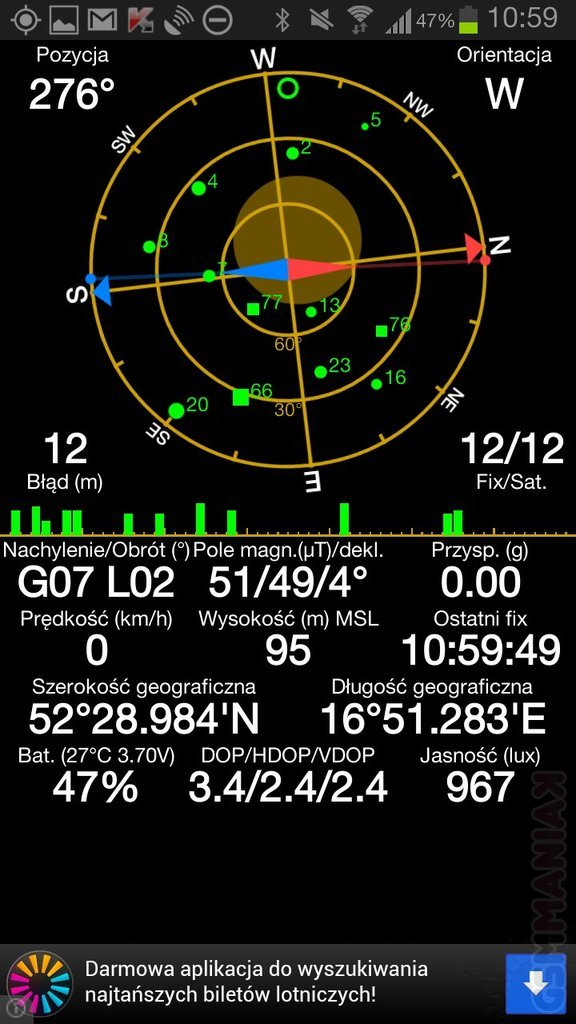
\includegraphics[scale=0.25]{czlonkowie/5/1ss.jpg}
\end{figure}
Prawdą jest, że odbiornik, który posiadamy w smartfonach to tak na prawdę A-GPS. Przedrostek “A” oznacza, że jest to system wspomagany przez sieć komórkową. Największym problemem jest prędkość znalezienia sygnału. Odbiorniki w smartfonach są małe, a w dodatku często używane w miastach gdzie są wysokie budynki, które nie pomagają w lokalizacji. Transmisja danych pozwala na pobranie danych, które dostarczają informacji modułowi GPS, w której części nieboskłonu ma szukać satelitów. W momencie kiedy połączenie z pierwszym zostanie ustanowione na podstawie porównań odbiornik znajdzie już pozostałe. Transmisja danych znacząco przyśpiesza połączenie z satelitami. Różnica między ustanowieniem lokalizacji bez transmisji danych, a z włączonym Internetem może wynosić 5-10 sekund do 3-5 minut. W najnowszych smartfonach jest już stosowany system Glonass. Jest to rosyjski odpowiednik GPS (amerykański). Korzystanie z dwóch odbiorników naraz poprawia dokładność i przyśpiesza wskazanie naszego położenia.
\begin{figure}[H]
\centering
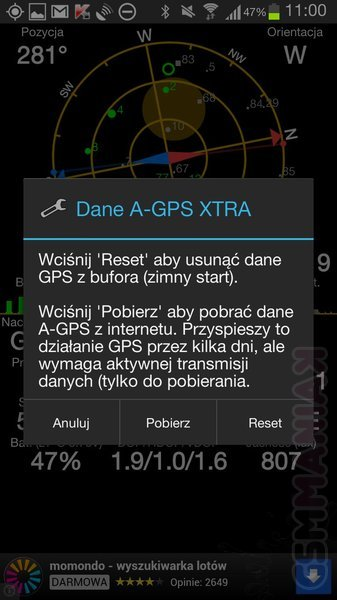
\includegraphics[scale=0.5]{czlonkowie/5/2ss.jpg}
\end{figure}
Drugim sposobem na lokalizację jest użycie sieci bezprzewodowej WiFi. Najważniejszym faktem jest, że nie musimy być połączeni z samą siecią, żeby udostępnić smartfonowi swoją pozycję. Skanuje on pobliskie sieci i na podstawie mocy sygnału (odległość od routera) określa nasze położenie. Ten typ lokalizacji nie jest dokładny ale przydaje się strasznie w budynkach, kiedy sygnał GPS lub Glonass jest niski lub nie ma go wcale. W praktyce dokładność lokalizacji jest na poziomie 200 m i większa. Wszystko zależy od ilości sieci WiFi w naszym otoczeniu.
\begin{figure}[H]
\centering

\includegraphics[scale=0.5]{czlonkowie/5/3ss.jpg}
\end{figure}
Trzecim sposobem jest lokalizacja na podstawie stacji bazowych sieci komórkowych tzw.BTS. Tu dokładność jest najmniejsza. Maszty operatorów mogą być oddalone od siebie nawet o kilka kilometrów. Zapewne pamiętacie w starych nokiach takie rozwiązania jak pokazywanie ulicy pod nazwą operatora. Jest to nadal realizowane właśnie na podstawie BTSów, które przesyłają dane do naszego smartfona. Cały szereg urządzeń takich jak akcelerometr, kompas, żyroskop czy barometr pomagają poprawić dokładność lokalizacji. Wspomagają one nawigację w ruchu. Ich użycie również wpływa na zmniejszenie zużycia energii w smartfonie poprzez ograniczenie korzystania z odbiornika GPS czy WiFi
\begin{figure}[H]
\centering
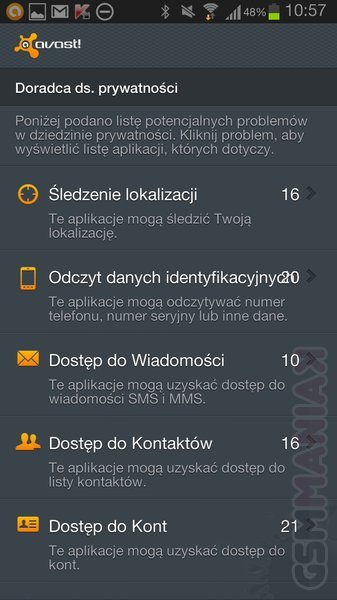
\includegraphics[scale=0.5]{czlonkowie/5/4ss.jpg}
\end{figure}
Liczba aplikacji, która korzysta z dostępu do lokalizacji jest ogromna. Czasami nawet możecie nie zdawać sobie z tego sprawy. Od taki program do korzystania z usług bankowych. Pozwala na sprawdzanie stanu konta, robienie przelewów czy przeglądanie historii. Jeśli nikt nie wchodził w dodatkowe opcje może się zdziwić skąd w wymaganych uprawnieniach tej aplikacji dostęp do lokalizacji. Na podstawie tych danych program jest wstanie wskazać nam najbliższe placówki banku oraz bankomaty. Zastanawiacie się pewnie czy to jest bezpieczne? Postanowiłem sobie zostawić ten temat na sam koniec.
\begin{figure}[H]
\centering
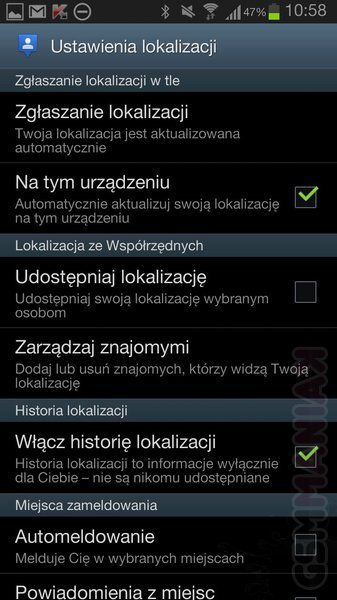
\includegraphics[scale=0.5]{czlonkowie/5/5ss.jpg}
\end{figure}
Ustawienia lokalizacji czy współrzędnych w Mapach Google są bardzo przydatnymi funkcjami. Dzięki nim nasi znajomi są nieustannie informowani gdzie się znajdujemy. Możemy w łatwy sposób znaleźć drogę do szukanego przez nas miejsca czy zlokalizować punkt użyteczności publicznej. Miejmy na uwadze, że ciągłe korzystanie z GPS oraz dzielenie się pozycją znacząco podnosi zużycie energii w smartfonie.
\begin{figure}[H]
\centering

\includegraphics[scale=0.5]{czlonkowie/5/6ss.jpg}
\end{figure}

\zadanieprojektowe{Czynniki wpływające na wynik pomiaru GPS, wady i zalety GPS}{2015-11-06}{2015-11-08}{zakończone}

Czynniki wpływające na wynik pomiaru GPS : \newline

******Satelity******
>>   Parametry orbity - dokładność wyznaczenia położenia
>>   środek fazowy anteny na satelicie
>>   pole grawitacyjne Ziemi
>>   opór atmosfery
>>   przyciąganie grawitacyjne ciał niebieskich (m.in. Słońca i Księżyca)
>>   oddziaływanie sił elektromagnetycznych
>>   ciśnienie światła słonecznego
>>   efekty relatywistyczne
     <>  OTW - ruch zegara w polu grawitacyjnym (zegar przyśpiesza o około 45.9 ns/doba)
     <>  STW - ruch zegara (zegar zwalnia około -7.2ns/doba)\newline

******Odbiorniki******
>>   niestabilność wzorców częstotliwości
>>   poprawki zegarów odbiorników
>>   cycle slip - nieciągłość fazy, czyli zmiana skokowa rejestrowanej fazy
>>   nieoznaczoność fazy
>>   środki fazowe anten odbiorników
>>   szum odbiornika
>>   rodzaj obserwacji - statyczne, kinematyczne, PPP
>>   odzyskiwanie fali nośnej L2 - dla pomiarów precyzyjnych\newline

******Zakłócenia propagacyjne******
>>   refrakcja troposfery i opóźnienie troposferyczne
>>   refrakcja jonosfery
>>   szumy atmosferyczne i kosmiczne
>>   odbicia i interferencja fal wtórnych\newline

******Zjawiska geofizyczne******
>>   nutacja
>>   ruch biegunów
>>   pływy skorupy ziemskiej
>>   pływy oceaniczne
>>   ruchy płyt tektonicznych
>>   oceaniczny efekt obciążeniowy\newline

******Pozostałe******
>>   nieciągłości fazy
>>   różnica czasu pomiędzy UT1 i UTC
>>   parametry transformacji między układami współrzędnych
>>   anti-spoofing (zapobieganie intencjonalnym próbom zakłócenia pracy systemu poprzez zmianę kodu P na Y)
>>   selective availability - zakłócanie sygnału cywilnego (czas i parametry satelity) pseudolosowym błędem - obecnie wyłączone\newline


Wady i zalety GPS \newline

Zalety:\newline

1.  Pomiary GPS są w zasadzie niezależne od warunków meteorologicznych na stanowiskach obserwacyjnych.\newline 


2.  Techniki obserwacyjne GPS nie wymagają wzajemnej widoczności obserwowanych punktów; wymagają natomiast odkrytego nieboskłonu od wysokości 150 od horyzontu. Nie jest zatem wymagana budowa specjalnych wież i stanowisk podwyższonych, jak to miało miejsce przy stosowaniu klasycznych technik naziemnych. Punkty sieci GPS można i należy lokalizować nie na trudno dostępnych wzgórzach, lecz w łatwo dostępnych miejscach przy szlakach komunikacyjnych. \newline \newline


3.  Pomiar satelitarny na stanowisku trwa bardzo krótko (pomiar statyczny dla punktów o znaczeniu lokalnym trwa około 45-60 minut, pomiar technologią szybką statyczną - 15-20 minut, zaś technologią "stop and go" tylko 1-2 minuty); dla niektórych prac geodezyjnych można stosować pomiary w czasie rzeczywistym (real time kinematic) dające wyniki natychmiast w terenie.\newline


4.  Dokładność pomiarów GPS jest na ogół wyższa od dokładności klasycznych metod obserwacyjnych. Przypomnijmy, że standardowa dokładność statycznych pomiarów względnych GPS wynosi 10-6.\newline


5.  Pomiar GPS na stanowisku jest w pełni zautomatyzowany. Wstępne opracowanie danych polowych może być opracowane od razu w terenie. Przy odpowiednio przygotowanym i realizowanym harmonogramie prac terenowych pełne opracowanie sieci może być prowadzone sukcesywnie.\newline


6.  Wyniki pomiarów GPS uzyskuje się w jednolitym geocentrycznym układzie współrzędnych globalnych. Poprzez nawiązanie pomiarów satelitarnych do istniejących punktów sieci krajowych uzyskuje się możliwość obliczenia parametrów transformacyjnych i współrzędnych wszystkich wyznaczanych punktów w układzie współrzędnych obowiązujących w danym kraju. Takie parametry transformacji są już wyznaczone dla układów współrzędnych obowiązujących w Polsce.\newline


7.  Wyznaczanie położenia punktów sieci metodami satelitarnymi GPS jest niezależne; nie występuje tu znane w klasycznej geodezji prawo przenoszenia się błędów w sieciach geodezyjnych.\newline


8.  Pomiary różnicowe GPS dostarczają jakościowo nowych elementów sieci, którymi są różnice współrzędnych X, Y, Z. Pomiary te dają zatem możność wyznaczenia zarówno skali jak i orientacji sieci.\newline


9.  Technologie pomiarów GPS są wysoce ekonomiczne. Koszt aparatury zwraca się bardzo szybko. Warto pamiętać, że koszt jednego odbiornika GPS wynosi tyle, ile kosztuje budowa 8-9 kilkunastometrowej wysokości wież triangulacyjnych.\newline

Wady:\newline

1.  Celowo wprowadzona degradacja sygnałów satelitów GPS powoduje znaczne zmniejszenie dokładności pomiarów bezwzględnych, a także różnicowych (względnych) w tych przypadkach, gdy użytkownik nie dysponuje odpowiednio zaawansowanymi odbiornikami, które mogą wyeliminować wpływ degradacji "anti-spoofing".\newline


2.  Niektóre technologie GPS wymagają nieprzerwanej łączności z satelitami podczas całej sesji pomiarowej (np. technologia "stop and 
go").\newline


3.  Występujące niekiedy zakłócenia w odbiorze sygnałów satelitarnych powodują przerwy w ciągłości pomiaru i tzw. utratę cykli. Fakt ten utrudnia opracowanie i wymaga dokonania najpierw rekonstrukcji cykli.\newline


4.  Satelity GPS dokonują dwóch obiegów wokół Ziemi w ciągu jednej doby. Powoduje to, że każdego dnia w określonym momencie czasu pojawia się taka sama konfiguracja satelitów GPS; pomiary wykonywane w tej samej porze dnia obarczone są zatem błędem konfiguracji geometrycznej konstelacji satelitów GPS.\newline%Ferdynand Sobieraj
 %Usuwa numeracje z naglowka. Zapewnia  dodanie do spisu tresci
\setcounter{secnumdepth}{-1}


%Gdy mamy dużą bibliografię to możemy wybierać pozycje,
%które cytujemy
%\nocite{ad-tg-80}

%Dodaje wszystkie pozycje z bibliografii
%\nocite{*}

%Po kazdym dodaniu nowej pozycji bibliograficznej
%z katalogu glownego uruchom: bibtex pracadyp
%\bibliographystyle{pdplain}
%\bibliography{tex/pracadyp}

\begin {thebibliography}{11}
\bibitem{Balcerzak2005} Balcerzak J., Pansiuk J.: \emph{Wprowadzenie do kartografii matematycznej}, Warszawa, OWPW~2005.
\bibitem{Barrett} Barrett R. i inni: \emph{Templates for the Solution of Linear Systems: Building Blocks for Iterative Methods1}, wersja elektorniczna Mathematics http://www.siam.org/books.
\bibitem{bjork} Bjork A., Dahlquist G.: \emph{Numerical Methods in Scientific Computing}, Philadelphia, SIAM~2002.
\bibitem{CCITTG4}CCITT, \emph{Facsimile Coding Schemes and Coding Control Functions for Group 4 Facsimile
Apparatus, Recommendation T.6, Volume VII, Fascicle VII.3, Terminal Equipment and
Protocols for Telematic Services, The International Telegraph and Telephone Consultative Committee (CCITT)}, Geneva, CCITT~1985.
\bibitem{drwal:mathematica2000} Drwal G, i in., \emph{Mathematica 4}, Gliwice, WPKJS~200.
\bibitem{Gdowski1982} Gdowski B.: \emph{Elementy geometrii rózniczkowej w zadaniach}, Warszawa, PWN~1982.
\bibitem{Gotlib2007} Gotlib D., Iwaniak A., Olszewski R.: \emph{GIS obszary zastosowań}, Warszawa, PWN~2007.
\bibitem{INTERGRAPHFileFormat1994} INTERGRAPH: \emph{INTERGRAPH RASTER FILE FORMAT REFERENCE GUIDE}, Alabama, Intergraph Corporation~1994.
\bibitem{Januszewski2006} Januszewski J.: \emph{Systemy satelitarne GPS, Galileo i inne}, Warszawa, PWN~2006.
\bibitem{kielbasinski1992}: Kiełbasiński A., Schwetlick H.: \emph{Numeryczna algebra liniowa}, Warszawa, WNT~1992.
\bibitem{Kincaid2006} Kincaid D.: \emph{Analiza numeryczna}, Warszawa, WNT~2006.
\bibitem{Lamparski2001}Lamparski J.: \emph{Navstar GPS od teorii do praktyki}, Olsztyn, WUW-M~2001.
\bibitem{Levine1994} Levine J.: \emph{Programowanie plików graficznych w C/C++}, New York, Wiley~1994.
\bibitem{Longley2006} Longley P. i inni: \emph{GIS teoria i praktyka}, Warszawa, PWN~2006.
\bibitem{GML:opengis} Open Geospatial Consortium Inc.: \emph{OpenGIS Geography Markup Language (GML) Encoding Standard, Version: 3.2.1},  OGC~2007.
\bibitem{GML:opengisimplemntation} Open Geospatial Consortium Inc.: \emph{OpenGIS® Geography Markup Language (GML) Implementation Specification}, OGC~2004.
\bibitem{Opera2002} Opera J.: \emph{Geometria róniczkowa i jej zastosowania}, Warszawa, PWN~2002.
\bibitem{Poczobut1982Geogeza} Odlanicki-Poczobut M.: \emph{Geodezja}, PPWK~1982.
\bibitem{Li2007}Li Y. i inni: \emph{GML Topology Data Storage Schema Design}, Chiba University~2007.
\bibitem{li2004GMLstorage}Li Y., Li J., Zhou S.: \emph{GML Storage}, A Spatial Database Approach,ER (Workshops), str 55-66, 2004.
\bibitem{Sayood2002} Sayood K.: \emph{Kompresja danych}, Warszawa, Rm~2002.
\bibitem{G52003} \emph{The Technical Instruction G-5, The Ground Cadastre and Buildings, The Main Surveying and
Cartographic Bureau}, Warszawa 2003.



\end {thebibliography}


\listoffigures

%\listoftables %Każdy członek zespołu musi dołożyć minimum 5 pozycji bibliograficzny, które posłużyły mu do opracowania zadanego fragmentu projektu.
\end{document}

To robi tylko kierownik projektu:
Wprowadź polecenie ze swoimi danymi
svn co https://riouxsvn.com/svn/zpi2014 --username aligeza

w bieżącym katalogu zostanie utworzony katalog z nazwą repozytorium, u mnie zpi2014

Skopiuj do niego całą zawartość projektu do katalogu zpi2014
przejdź do niego i wprowadź
svn add * --force
to polecenie dodało wszystkie pliki i podkatalogu do lokalnej kopii repozytorium.


Poniższe polecenie wyśle dane na serwer svn
svn commit -m "inicjacja dokumentacji projektu"


Teraz każdy członek z zespołu wykonuje polecnie ze swoim loginem!!!!!!!
Wprowadź polecenie ze swoimi danymi
svn co https://riouxsvn.com/svn/zpi2014 --username aligeza
Już każdy posiada swoje repozytorium do kompilacji.
Zmiany nanosić w swoim pliku i po porawnej kompilacji
trzeba przesłać na serwer z adekwatnym komentarzem
svn commit -m "Model stanowiska do zobrazowań"